
    \begin{enumerate}[label=(\alph*)]
    \item
    Khi chậu M đặt tại gốc tọa độ O $\left(0, 0\right)$ là trọng tâm của bàn, vì các dây treo là giống nhau nên trọng lực kéo căng các dây là bằng nhau.
    \\
    Lực căng các dây là:
    \begin{equation}
        T_1= T_2= T_3=T_4=T.
    \end{equation}
    Điệu kiện cân bằng là tổng các lực căng phải có độ lớn bằng trọng lực hệ vật:
    \begin{equation}
        |\vec{T_1}| + |\vec{T_2}| + |\vec{T_3}| +|\vec{T_4}| = |\vec{P}|.
    \end{equation}
    \begin{equation}    
        \Longrightarrow 4T = (m+M)\cdot g.
    \end{equation}
    \begin{equation}   
        \boxed{
        \Longrightarrow T = \dfrac{(m+M)\cdot g}{4}.
        }
    \end{equation}
    \item 
    \begin{enumerate}[label=(\roman*)]
    \item
        \begin{figure}[H]
    \centering
    \tikzset{every picture/.style={line width=0.75pt}} %set default line width to 0.75pt        

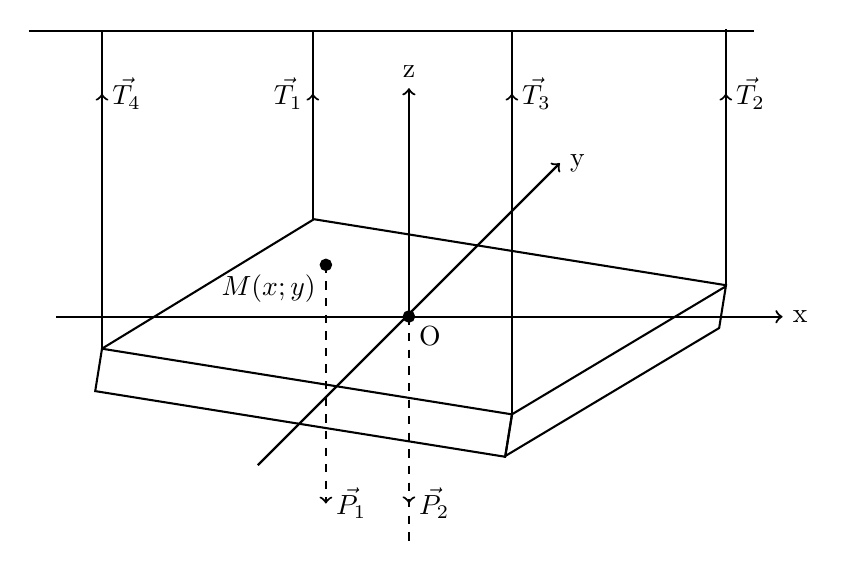
\begin{tikzpicture}[x=0.75pt,y=0.75pt,yscale=-1,xscale=1]
%uncomment if require: \path (0,429); %set diagram left start at 0, and has height of 429

%Shape: Rectangle [id:dp43479829147458826] 
\draw   (147.34,176.52) -- (344.82,208.15) -- (341.55,228.58) -- (144.07,196.95) -- cycle ;
%Shape: Rectangle [id:dp26418096458424434] 
\draw   (344.94,208.08) -- (447.9,146.46) -- (444.68,166.56) -- (341.71,228.19) -- cycle ;
%Straight Lines [id:da6303516163988201] 
\draw    (248.92,114.05) -- (448.42,146) ;
%Straight Lines [id:da2435007903542885] 
\draw    (147.3,176.51) -- (249.25,114.27) ;
%Shape: Rectangle [id:dp43479829147458826] 
%\draw   (150,200) -- (350,200) -- (350,220) -- (150,220) -- cycle ;
%Shape: Rectangle [id:dp26418096458424434] 
%\draw   (350,200) -- (442.03,122.78) -- (442.03,143.14) -- (350,220) -- cycle ;
%Straight Lines [id:da6303516163988201] 
%\draw    (240.42,122.25) -- (442.46,122.25) ;
%Straight Lines [id:da2435007903542885] 
%\draw    (149.96,200) -- (240.78,122.42) ;
%WALL 
\draw    (112.03,23.59) -- (461.43,23.59) ;
%Shape: Axis 2D [id:dp11255839884999319] 
%\draw [dashed] (121.01,156.7) -- (506.99,156.7)(409.6,45.33) -- (177.57,277.36) (504.99,151.7) -- (506.99,156.7) -- (494.99,161.7) (397.6,52.33) -- (409.6,45.33) -- (407.6,52.33)  ;
%Straight Lines [id:da6910540327628811] 
\draw  [->]  (147.34,176.52) -- (147.34,53.64) node [right] {$\vec{T_4}$} ;
\draw    (147.34,176.52) -- (147.34,23.64) ;
%Straight Lines [id:da778712219228807] 
\draw  [->]  (248.92,114.27) -- (248.92,53.64) node [left] {$\vec{T_1}$} ;
\draw    (248.92,114.27) -- (248.92,23.55) ;
%Straight Lines [id:da014093703911455924]
\draw  [->]  (447.9,146.46) -- (447.9,53.64) node [right] {$\vec{T_2}$} ;
\draw    (447.9,146.46) -- (447.9,22.35) ;
%Straight Lines [id:da13741894893199325] 
\draw    (344.82,200) -- (344.82,104.51) -- (344.82,23.64) ;
\draw  [->]  (344.82,208.15) -- (344.82,53.64) node [right] {$\vec{T_3}$} ;


% Text Node

\filldraw(255.21,136.12) circle(2.5)node [anchor=north east][align=right] {$M(x;y)$};
\draw[dashed][->](255.21,136.12) -- (255.21,251.12) node [right]{$\vec{P_1}$};

\draw[thick]  [->] (125.23,161.12) -- (475.23,161.12) node [right]{x};
\draw[ thick]  [->] (222.42,232.62) -- (367.93,87.11) node [right] {y};
\draw[ thick] [dashed](295.21,161) -- (295.21,271);
\draw [dashed][->](295.21,201) -- (295.21,251) node [right] {$\vec{P_2}$};
\draw[ thick]  [->] (295.21,161) -- (295.21,51) node [above] {z};
\filldraw(295.21,161) circle(2.5) node [anchor=north west][align=left] {O};
\end{tikzpicture}
    \caption{}
    \label{fig:S4_01}
    \end{figure}
    Chậu M được coi là chất điểm đặt tại $M \left( x;y \right)$ với hệ trục tọa độ gắn với khối tâm của bàn nằm ngang.
    Các điều kiện cân bằng của hệ vật:
    \begin{enumerate} [label=(\arabic*)]
    \item Cân bằng lực theo phương thẳng đứng: Tổng độ lớn các lực căng dây phải bằng trọng lượng của hệ vật:
    \begin{equation}
        \vec{T_1} + \vec{T_2} + \vec{T_3} +\vec{T_4} = \vec{P}.
    \end{equation}
    Tức:
    \begin{equation}
        |\vec{T_1}| + |\vec{T_2}| + |\vec{T_3}| +|\vec{T_4}| = |\vec{P}|.
    \end{equation}
    hay:
    \begin{equation}
        T_1+T_2+T_3+T_4 = (m+M) \cdot g.
    \end{equation}
        \item
    Tính đàn hồi của dây:
    Vì hệ số đàn hồi của dây K là rất lớn và giới hạn đàn hồi không đáng kể, bàn chuyển dịch một đoạn rất nhỏ theo phương thẳng đứng.
    \\
    Xét sự chuyển vị theo phương thẳng đứng (Oz) tại mỗi đỉnh của bàn:
            \begin{figure}[H]
    \centering
    \tikzset{every picture/.style={line width=0.75pt}} %set default line width to 0.75pt        
\begin{tikzpicture}
       \node (a) at (0,0)
         {
\begin{tikzpicture}[x=0.75pt,y=0.75pt,yscale=-1,xscale=1]
\draw [->] (165.23,161.12) -- (435.23,161.12) node [right]{y};
\draw(295.21,161) -- (295.21,271);
\draw [->] (295.21,161) -- (295.21,51) node [above] {z};
%\draw (295.21,161) circle (7.5);
%\draw (295.21,161)node[anchor=south east] {x};
\filldraw(295.21,161) circle(2.5) node [anchor=north west][align=left] {O};
\draw   (200,175) -- (400,200) -- (400,205) -- (200,180) -- cycle ;
\draw[dashed](400,205.5) -- (295.21,205.5) node[left]{$z_y$};
\draw (295.21,180) node[left] {$z_0$};
\draw
(210,176) to [in=5](210,161.12);
\draw
(215,176.5) to [in=5](215,161.12)
;
\draw (220,171.12) node [right] {$\theta y$};
\draw [dashed] [<->](400,205) -- (400,161.12);
\draw (400, 180) node[right]{$\Delta z_x$};
\end{tikzpicture}
};
\node (b) at (a.east) [xshift=150]
{
%\end{tikzpicture}
%    \caption{}
%    \label{fig:S4_02}
%    \end{figure}
%            \begin{figure}[H]
%    \centering
    \tikzset{every picture/.style={line width=0.75pt}} %set default line width to 0.75pt        

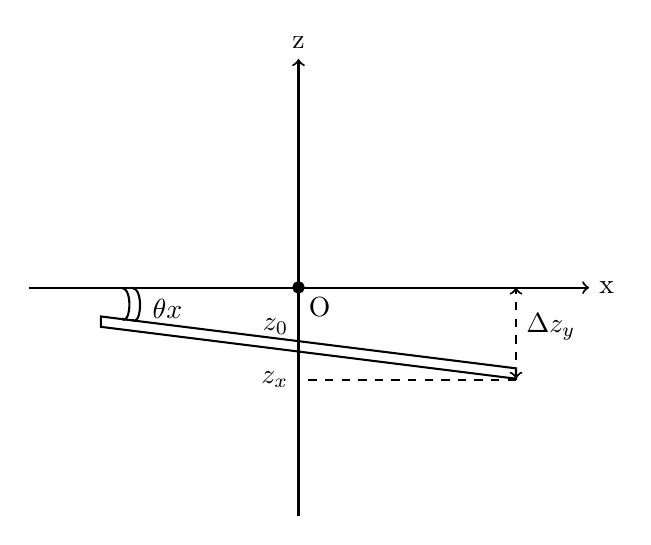
\begin{tikzpicture}[x=0.75pt,y=0.75pt,yscale=-1,xscale=1]
\draw [->] (165.23,161.12) -- (435.23,161.12) node [right]{x};
\draw(295.21,161) -- (295.21,271);
\draw [->] (295.21,161) -- (295.21,51) node [above] {z};
%\draw (295.21,161) circle (7.5) 
%\draw (295.21,161) node[anchor=south east] {y};
\filldraw(295.21,161) circle(2.5) node [anchor=north west][align=left] {O};
\draw   (200,175) -- (400,200) -- (400,205) -- (200,180) -- cycle ;
\draw
(210,176) to [in=5](210,161.12);
\draw
(215,176.5) to [in=5](215,161.12)
;
\draw (220,171.12) node [right] {$\theta x$};
\draw[dashed](400,205.5) -- (295.21,205.5);
\draw (295.21,205.5) node[left]{$z_x$};
\draw [dashed] [<->](400,205) -- (400,161.12);
\draw (400, 180) node[right]{$\Delta z_y$};
\draw (295.21,180) node[left] {$z_0$};
\end{tikzpicture}
 };
 \end{tikzpicture}
    \caption{}
    \label{fig:S4_02}
    \end{figure}
    Vì góc nghiêng của bàn rất nhỏ và có thể xem như không nghiêng, ta có thể xem sự chuyển vị là tuyến tính:
    \\Tại vị trí $\left(-\dfrac{a}{2};\dfrac{a}{2}\right)$:
    \begin{equation}
        \Delta z_1 = z_0 +\dfrac{a}{2} \theta y -\dfrac{a}{2} \theta x.
    \end{equation}
    Tại vị trí $\left(\dfrac{a}{2};\dfrac{a}{2}\right)$:
    \begin{equation}
        \Delta z_2 = z_0 +\dfrac{a}{2} \theta y +\dfrac{a}{2} \theta x.
    \end{equation}
    Tại vị trí $\left(\dfrac{a}{2};-\dfrac{a}{2}\right)$:
    \begin{equation}
        \Delta z_3 = z_0 -\dfrac{a}{2} \theta y 
 +\dfrac{a}{2} \theta x.
    \end{equation}
    Tại vị trí $\left(-\dfrac{a}{2};-\dfrac{a}{2}\right)$:
    \begin{equation}
        \Delta z_4 = z_0 -\dfrac{a}{2} \theta y -\dfrac{a}{2} \theta x.
    \end{equation}
    Áp dụng định luật Hooke cho các dây treo dãn đã cho, lực căng dây i có độ lớn:
    \begin{equation}
        T_i = k \cdot \Delta z_i \left( i \in N^* |1 \le i \le 4 \right).
    \end{equation}
    với độ dãn của dây là $\Delta z_i$.
    \item Do độ nghiêng của bàn là nhỏ, ta bỏ qua momen gây bởi lực ma sát nghỉ sinh ra để giữ cân bằng cho vật, có độ lớn tỉ lệ với góc nghiêng. \newline Momen lực gây ra bởi các lực căng dây có thể được phân tích thành hai thành phần.
    \newline
    Cân bằng moment lực đối với M trên trục Ox:
    \begin{equation}
        \dfrac{a}{2}\vec{T_1}+\dfrac{a}{2}\vec{T_2}+\dfrac{a}{2}\vec{T_3}+\dfrac{a}{2}\vec{T_4} =  |y|\cdot \vec{P_1}.
    \end{equation}
    Trên trục Ox:
    \begin{equation}
    \Longrightarrow    
    -\dfrac{a}{2}T_1+\dfrac{a}{2}T_2+\dfrac{a}{2}T_3-\dfrac{a}{2}T_4 = Mgy.
    \end{equation}
    \begin{equation}
    \Longleftrightarrow   
    T_2 +T_3 - T_1-T_4 = \dfrac{2Mgy}{a}.
    \end{equation}
    \item
    Cân bằng moment đối với vật M trên trục Oy:
    \begin{equation}
        \dfrac{a}{2}\vec{T_1}+\dfrac{a}{2}\vec{T_2}+\dfrac{a}{2}\vec{T_3}+\dfrac{a}{2}\vec{T_4} =  |x|\cdot \vec{P_1}.
    \end{equation}
    Trên trục Oy:
    \begin{equation}
    \Longrightarrow    
    -\dfrac{a}{2}T_1-\dfrac{a}{2}T_2+\dfrac{a}{2}T_3+\dfrac{a}{2}T_4 = Mgx.
    \end{equation}
    \begin{equation}
    \Longleftrightarrow   
    T_3 +T_4- T_1-T_2 = \dfrac{2Mgx}{a}.
    \end{equation}
    \end{enumerate}
    Kết hợp điều kiện (1.):
    \begin{equation}
        T_1 + T_2 +T_3 +T_4 = k \cdot (z_1 +z_2+z_3+z_4) = k \cdot 4z_0 = (m+M)\cdot g.
    \end{equation}
    Do vậy:
    \begin{equation}
        z_0 = \dfrac{(m+M)\cdot g}{4k}.
    \end{equation}
    Kết hợp điều kiện (2.):
    \begin{equation}
        T_2 +T_3 - T_1 -T_4 = k \cdot (z_2 +z_3 - z_1 - z_4)
    \end{equation}
    \begin{equation} 
        = k \cdot \left[(a \cdot \theta y + a \cdot \theta x) + (-a \cdot \theta y + a \cdot \theta x) - (a \cdot \theta y - a \cdot \theta x) - (-a \cdot \theta y - a \cdot \theta x)\right]
    \end{equation}
    \begin{equation}
        = k \cdot 2a \theta y = \dfrac{2Mgy}{a}.
    \end{equation}
    Vì thế:
    \begin{equation}
        \theta y = + \dfrac{Mgy}{ka^2}.
    \end{equation}
    Kết hợp điều kiện (3.):
    \begin{equation}
        T_3 +T_4 - T_1 -T_2 = k \cdot (z_3 +z_4 - z_1 - z_2)
    \end{equation}
    \begin{equation} 
        = k \cdot \left[(-a \cdot \theta y + a \cdot \theta x) + (-a \cdot \theta y - a \cdot \theta x) - (a \cdot \theta y - a \cdot \theta x) - (a \cdot \theta y + a \cdot \theta x)\right]
    \end{equation}
    \begin{equation}
        = k \cdot 2x \theta y = \dfrac{2Mgx}{a}.
    \end{equation}
    Vì thế:
    \begin{equation}
        \theta x = + \dfrac{Mgx}{ka^2}.
    \end{equation}
    Từ $z_0 = \dfrac{(m +M)\cdot g}{4k}$; $\theta y = \dfrac {Mgy}{ka^2}$; $\theta x = \dfrac {Mgx}{ka^2}$ thế vào biểu thức lực căng từ dây $T_i=k \cdot \Delta z_i$, ta được:
    
    \begin{equation}
    \boxed{
        T_1 = k \cdot \left[ \dfrac{(m+M)g}{4k}+\dfrac{a}{2} \cdot \dfrac{Mgy}{ka^2}-\dfrac{a}{2}\cdot \dfrac{Mgx}{ka^2}\right] = \dfrac{(m+M)g}{4}+\dfrac{Mgy}{2a}-\dfrac{Mgx}{2a}.
            }
    \end{equation}
    \begin{equation}
    \boxed{
        T_2 = k \cdot \left[ \dfrac{(m+M)g}{4k}+\dfrac{a}{2} \cdot \dfrac{Mgy}{ka^2}+\dfrac{a}{2}\cdot \dfrac{Mgx}{ka^2}\right] = \dfrac{(m+M)g}{4}+\dfrac{Mgy}{2a}+\dfrac{Mgx}{2a}.
            }
    \end{equation}
    \begin{equation}
    \boxed{
        T_3 = k \cdot \left[ \dfrac{(m+M)g}{4k}-\dfrac{a}{2} \cdot \dfrac{Mgy}{ka^2}+\dfrac{a}{2}\cdot \dfrac{Mgx}{ka^2}\right] = \dfrac{(m+M)g}{4}-\dfrac{Mgy}{2a}+\dfrac{Mgx}{2a}.
            }
    \end{equation}
    \begin{equation}
    \boxed{
        T_4 = k \cdot \left[ \dfrac{(m+M)g}{4k}-\dfrac{a}{2} \cdot \dfrac{Mgy}{ka^2}-\dfrac{a}{2}\cdot \dfrac{Mgx}{ka^2}\right] = \dfrac{(m+M)g}{4}-\dfrac{Mgy}{2a}-\dfrac{Mgx}{2a}.
            }
    \end{equation}
\item Dây sẽ bị chùng khi không có lực nào căng hai đầu dây. Vì bàn có khối lượng $m>0$ nên không có trường hợp hai dây trùng một lúc.
\\$\longrightarrow$ Chỉ một dây có thể trùng một lúc, tức $T_i \le 0$
Với $i =1$ (Dây 1 bị trùng), $T_1 \le 0$:
\begin{equation}
\Longrightarrow\dfrac{(m+M)g}{4}+\dfrac{Mgy}{2a}-\dfrac{Mgx}{2a} \le 0.
\end{equation}
\begin{equation}
\label{eq:S4_01}
\Longrightarrow
y \le x -\dfrac{(m+M)a}{2M}.
\end{equation}
Với $i =2$, $T_2 \le 0$:
\begin{equation}
\Longrightarrow\dfrac{(m+M)g}{4}+\dfrac{Mgy}{2a}+\dfrac{Mgx}{2a} \le 0.
\end{equation}
\begin{equation}
\label{eq:S4_02}
\Longrightarrow
y \le -x -\dfrac{(m+M)a}{2M}.
\end{equation}
Với $i =3$, $T_3 \le 0$:
\begin{equation}
\Longrightarrow\dfrac{(m+M)g}{4}-\dfrac{Mgy}{2a}+\dfrac{Mgx}{2a} \le 0.
\end{equation}
\begin{equation}
\label{eq:S4_03}
\Longrightarrow
y \ge x + \dfrac{(m+M)a}{2M}.
\end{equation}
Với $i =4$, $T_4 \le 0$:
\begin{equation}
\Longrightarrow\dfrac{(m+M)g}{4}-\dfrac{Mgy}{2a}-\dfrac{Mgx}{2a} \le 0.
\end{equation}
\begin{equation}
\label{eq:S4_04}
\Longrightarrow
y \ge -x + \dfrac{(m+M)a}{2M}.
\end{equation}
Tập hợp điểm M đặt chậu trên bàn là hình vuông tạo bởi các đỉnh:
\\$\left(-\dfrac{a}{2},\dfrac{a}{2}\right)$;$\left(\dfrac{a}{2},\dfrac{a}{2}\right)$;$\left(\dfrac{a}{2};\dfrac{a}{2}\right)$;$\left(-\dfrac{a}{2},\dfrac{a}{2}\right)$.
Xét $i=4$ (dây 4 bị trùng là trường hợp điển hình)
\begin{equation}
   \begin{cases}
   y = -x + \dfrac{(m+M)a}{2M}
   \\
   y=\dfrac{a}{2}
   \end{cases}
\end{equation}
\begin{equation}
    \Longrightarrow x=\dfrac{a}{2}\cdot \dfrac{m}{M}.
\end{equation}
\begin{equation}
   \begin{cases}
   y = -x + \dfrac{(m+M)a}{2M}
   \\
   x=\dfrac{a}{2}
   \end{cases}
\end{equation}
\begin{equation}
    \Longrightarrow y=\dfrac{a}{2}\cdot \dfrac{m}{M}.
\end{equation}
$\Longrightarrow$ $\begin{cases}
\text{M nằm ngoài bàn: $m>M;m,M>0$}
\\
\text{M thỏa mãn: $m \le M ;m,M >0$}
\end{cases}$
\\
Ta thấy rằng:
\\Với $m>M$ (bàn có khối lượng lớn hơn chậu cây) thì không có vị trí đặt trên bàn chậu M để dây bị chùng.
\\ Với $m=M$, các điểm thỏa mãn là các đỉnh treo dây của bàn.
\\Nếu bàn có khối lượng $m<M$, quỹ tích điểm $M(x;y)$ thỏa mãn đề bài là vùng giao nhau trong không gian bàn với các bất phương trình \eqref{eq:S4_01}, \eqref{eq:S4_02}, \eqref{eq:S4_03}, \eqref{eq:S4_04}.

\begin{figure}[H]
    \centering
    \tikzset{every picture/.style={line width=0.75pt}} %set default line width to 0.75pt       
\begin{tikzpicture}[x=0.75pt,y=0.75pt,yscale=-1,xscale=1]
\draw [->] (115.23,161.12) -- (485.23,161.12) node [right]{x};
\draw(295.21,161) -- (295.21,321);
\draw [->] (295.21,161) -- (295.21,1) node [above] {y};
\draw (295.21,161) circle (7.5) node[anchor=south west] {z};
\filldraw(295.21,161) circle(2.5) node [anchor=south east] {O};
\draw (395.21,61) -- (395.21,261)--(195.21,261)--(195.21,61)--(395.21,61);
\draw[dashed] (420.21,161)--(295.21,36)--(170.21,161)--(295.21,286)--(420.21,161);
\filldraw [fill=gray!20] (195.21,185.12) -- (195.21,261) -- (271,261);
\filldraw [fill=gray!20] (395.21,185.12) -- (395.21,261) -- (319,261);
\filldraw [fill=gray!20] (195.21,137) -- (195.21,61) -- (271,61);
\filldraw [fill=gray!20] (395.21,137) -- (395.21,61) -- (319,61);
\filldraw(295.21,36) circle(2.5) node [anchor=south east] {$y_i$};
\filldraw(420.21,161) circle(2.5) node [anchor=north west] {$x_i$};
\filldraw(195.21,161) circle(1.25) node [anchor=south west] {$-\dfrac{a}2$};
\filldraw(395.21,161) circle(1.25);
\draw (385.21,161) node [anchor=north east]{$\dfrac{a}2$};
\filldraw(295.21,261) circle(1.25) node [anchor=south west] {$-\dfrac{a}2$};
\filldraw(295.21,61) circle(1.25) node [anchor=north east] {$\dfrac{a}2$};
\filldraw(295.21,286) circle(1.25);
\draw (295.21,300) node [anchor=south west] {$-a$};
\filldraw (319,61) circle(1.25) node [anchor=south west] {$\left( \dfrac{a}2 \dfrac{m}{M};\dfrac{a}2 \right)$};
\filldraw (395.21,137) circle(1.25);
\draw (395.21,130)node [right] {$\left( \dfrac{a}2 \dfrac{m}{M};\dfrac{a}2 \right)$};
\end{tikzpicture}
    \caption{
    $\begin{cases}
    \dfrac{a}2 \le |x_i| \le a
    \\
    \\
    \dfrac{a}2 \le |y_i| \le a
    \end{cases}
    $
    ($x_i,y_1$ là giao điểm bất phương trình dây i với trục Ox, Oy)
    }
    \label{fig:S4_03}
    \end{figure}
Nhận xét: Lực căng dây có độ lớn cỡ trọng lượng của bàn. Lực ma sát tỉ lệ với độ nghiêng với khối lượng của chậu. Vậy nếu khối lượng chậu rất nhỏ so với bàn, lực ma sát do đó sẽ vô cùng bé và mô hình ta hoạt động tốt.
    \item
    Dây sẽ bị đứt khi lực căng hai đầu dây vượt qua lực căng tối đa dây có thể chịu $T_{\text{i max}} = \Delta l_0 \cdot k$. Khi đó $M(x;y)$ đặt chậu cân bằng khi $T_i \le \Delta l_0 \cdot k$.
    \\
    Với $i=1$:
    \begin{equation}
        T_1 \le \Delta l_0 \cdot k
    \end{equation}
    \begin{equation}
        \Longrightarrow \dfrac{(m+M)g}4 + \dfrac{Mg}{2a} (y-x)\le k \cdot \Delta l_0.
    \end{equation}
    \begin{equation}
    \label{eq:S4_05}
        \Longrightarrow y - x \le \dfrac{2ak\Delta l_0}{Mg}-\dfrac{(m+M)a}{2M} = \dfrac {a \left[4k \Delta l_0 - (m+M)g\right]}{2Mg}.
    \end{equation}

    Với $i=2$:
    \begin{equation}
        T_2 \le \Delta l_0 \cdot k
    \end{equation}
    \begin{equation}
        \Longrightarrow \dfrac{(m+M)g}4 + \dfrac{Mg}{2a} (y+x)\le k \cdot \Delta l_0.
    \end{equation}
    \begin{equation}
    \label{eq:S4_06}
        \Longrightarrow y - x \le  \dfrac {a \left[4k \Delta l_0 - (m+M)g\right]}{2Mg}.
    \end{equation}

    Với $i=3$:
    \begin{equation}
        T_3 \le \Delta l_0 \cdot k
    \end{equation}
    \begin{equation}
        \Longrightarrow \dfrac{(m+M)g}4 + \dfrac{Mg}{2a} (x-y)\le k \cdot \Delta l_0.
    \end{equation}
    \begin{equation}
    \label{eq:S4_07}
        \Longrightarrow x - y \le  \dfrac {a \left[4k \Delta l_0 - (m+M)g\right]}{2Mg}.
    \end{equation}

    Với $i=4$:
    \begin{equation}
        T_4 \le \Delta l_0 \cdot k
    \end{equation}
    \begin{equation}
        \Longrightarrow \dfrac{(m+M)g}4 + \dfrac{Mg}{2a} (-x-y)\le k \cdot \Delta l_0.
    \end{equation}
    \begin{equation}
    \label{eq:S4_08}
        \Longrightarrow -x - y \le  \dfrac {a \left[4k \Delta l_0 - (m+M)g\right]}{2Mg}.
    \end{equation}
Kết hợp với tập hợp $M(x;y)$ trên bàn:
\\ Xét $i=2$ (Trường hợp dây 2 đứt làm điển hình):
\begin{equation}
    \begin{cases}
       y - x =  \dfrac {a \left[4k \Delta l_0 - (m+M)g\right]}{2Mg}
       \\
       x = \dfrac{a}2
    \end{cases}
\Longrightarrow y =  \dfrac {a \left[4k \Delta l_0 - mg\right]}{2Mg}.
\end{equation}
\begin{equation}
    \begin{cases}
       y - x =  \dfrac {a \left[4k \Delta l_0 - (m+M)g\right]}{2Mg}
       \\
       y = \dfrac{a}2
    \end{cases}
\Longrightarrow x =  \dfrac {a \left[4k \Delta l_0 - mg\right]}{2Mg}.
\end{equation}
Với $k, \Delta l_0$ đã cho thỏa mãn, quỹ tích các điểm $M(x;y)$ đặt chậu cân bằng trên mặt bàn là giao nhau các bất phương trình \eqref{eq:S4_05}, \eqref{eq:S4_06}, \eqref{eq:S4_07}, \eqref{eq:S4_08} với mặt bàn:
            \begin{figure}[H]
    \centering
    \tikzset{every picture/.style={line width=0.75pt}} %set default line width to 0.75pt        
\begin{tikzpicture}
       \node (a) at (0,0)
         {

\begin{tikzpicture}[x=0.5pt,y=0.5pt,yscale=-1,xscale=1]
\filldraw [fill=gray!20] (295.21,84.825) -- (371,161.12)--(295.21,237.125)--(219.21,161.12);
\draw [->] (115.23,161.12) -- (485.23,161.12) node [right]{x};
\draw(295.21,161) -- (295.21,321);
\draw [->] (295.21,161) -- (295.21,1) node [above] {y};
\draw (295.21,161) circle (7.5) node[anchor=south west] {z};
\filldraw(295.21,161) circle(2.5) node [anchor=south east] {O};
\draw (395.21,61) -- (395.21,261)--(195.21,261)--(195.21,61)--(395.21,61);
\draw[dashed] (395.21,137) -- (271,261);
\draw (295.21,84.825) circle (1.25)node[right]{$y_i$};
\draw (371,161.12) circle (1.25)node[above]{$x_i$};
\filldraw  (319,61) circle(1.25);
\draw (319,61)node[anchor = south west]{$\left( x;\dfrac{a}2 \right)$};
\filldraw  (395.21,137) circle(1.25);
\draw (395.21,137)node[anchor = south west]{$\left( \dfrac{a}2 ;y\right)$};
\draw[dashed] (319,61) -- (195.21,185.12);
\draw[dashed] (271,61) -- (395.21,185.12);
\draw[dashed] (195.21,137) -- (319,261);

\draw (295.21,84.825)--(219.21,161.12);
\draw (295.21,237.125)--(219.21,161.12);
\draw (295.21,237.125) -- (371,161.12);
\draw (295.21,84.825) -- (371,161.12);

\end{tikzpicture}


};
\node (b) at (a.east) [xshift=150]
{

\begin{tikzpicture}[x=0.5pt,y=0.5pt,yscale=-1,xscale=1]
\filldraw [fill=gray!20] (420.21,161)--(295.21,36)--(170.21,161)--(295.21,286)--(420.21,161);
\filldraw [fill=gray!80] (319,61)--(395.21,137)--(395.21,185.5)--(320,261)--(270,261)--(195,185.5)--(195,137)--(270,61);
\draw [->] (115.23,161.12) -- (485.23,161.12) node [right]{x};
\draw(295.21,161) -- (295.21,321);
\draw [->] (295.21,161) -- (295.21,1) node [above] {y};
\draw (295.21,161) circle (7.5) node[anchor=south west] {z};
\filldraw(295.21,161) circle(2.5) node [anchor=south east] {O};
\draw (395.21,61) -- (395.21,261)--(195.21,261)--(195.21,61)--(395.21,61);

\filldraw(295.21,36) circle(2.5) node [anchor=south east] {$y_i$};
\filldraw(420.21,161) circle(2.5) node [anchor=north west] {$x_i$};
\filldraw (319,61) circle(1.25) node [anchor=south west] {$\left( x;\dfrac{a}2 \right)$};
\filldraw (395.21,137) circle(1.25);
\draw (395.21,125)node [right] {$\left( y;\dfrac{a}2 \right)$};
\end{tikzpicture}

 };
 \end{tikzpicture}
    \label{fig:S4_04}
    \caption{ Quỹ tích các điểm $M(x;y)$ lần lượt trong các trường hợp
    $\left( k \cdot \Delta l_0 < \dfrac{(m+M)g}{4} \right)$
    và
    $\left( k \cdot \Delta l_0 > \dfrac{(m+M)g}{4} \right)$ với $x_i$ và $y_i$ là 
     giao điểm bất phương trình dây i Với trục Ox, Oy.
    }
    \end{figure}
    Khi $k \cdot \Delta l_0 = \dfrac{(m+M)g}{4}$ thì quỹ tích là không gian trong hình thoi nội tiếp của bàn với các đỉnh lần lượt là trung điểm các cạnh bàn.
    \end{enumerate}
    \end{enumerate}
    \newpage
\textbf{Phổ điểm}
    \begin{center}
    \begin{tabular}{|c|p{8cm}|c|}
    \hline
    \multicolumn{1}{|l|}{Phần} & Nội dung & Điểm thành phần \\ 
    \hline
\multirow{1}{*}{(a)} & Chứng minh được công thức đã cho.
                     & 0.75
                     \\
                     \hline  
\multirow{1}{*}{(b)(i)} & Chỉ ra 4 điều kiện cân bằng.                                  
                     & 1    
                     \\
                     \cline{2-3}
                     & Kết hợp các điều kiện vào suy ra $\theta x$. 
                     & 0.5
                     \\
                     \cline{2-3}
                     & Ra được các biểu thức xác định $T_i$. 
                     & 0.5
                     \\
                     \hline
\multirow{1}{*}{(b)(ii)}& Ra được các bất đẳng thức xác định $x$ và $y$ của từng dây
                     & 0.25    
                     \\
                     \cline{2-3}
                     & Biện luận về m và M
                     & 0.25
                     \\
                     \cline{2-3}
                     & Ra được quỹ tích điểm $M(x;y)$
                     & 0.25
                     \\
                     \hline
\multirow{1}{*}{(b)(iii)}& Điều kiện của $T_i$ khi dây bị đứt
                     & 0.25    
                     \\
                     \cline{2-3}
                     & Ra được quỹ tích điểm $M(x;y)$ trong trường hợp này
                     & 0.25
                     \\
                     \hline
    \end{tabular}
    \end{center}